\chapter{Uvod}
    Projekt FERSAT, koji se od 2018. godine provodi na Fakultetu elektrotehnike i računarstva, uključuje izradu i lansiranje satelita CubeSat te korištenje satelita u svrhu prikupljanja informacija o svjetlosnom zagađenju i debljini ozonskog omotača, fotografiranja površine Zemlje i horizonta, te ispitivanja sustava za komunikaciju u radijskom X-pojasu. Satelit u izradi dimenzija je približno 10 cm x 10 cm x 10 cm, volumena jedne litre i ne teži od 4/3 kilograma, što ga svrstava u skupinu satelita formata CubeSat 1U \cite{fersat_stranica_projekta}. Očekivani životni vijek satelita je 3 godine, a bit će postavljen u niskoj Zemljinoj orbiti na visini između 500 i 600 kilometara. Slika \ref{fig:fersat} prikazuje planirani izgled satelita.
    
    \begin{figure}[htb]
        \centering
        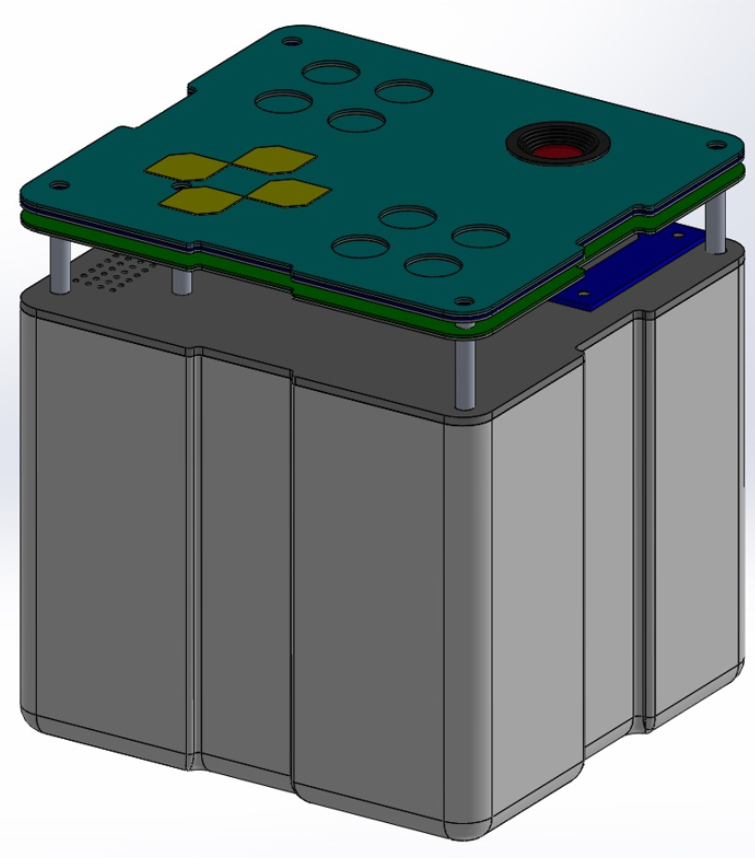
\includegraphics[height=7cm]{slike/fersat.png}
        \caption{Skica planiranog izgleda FERSAT-a. Prikazani su korisni teret \engl{payload} i platforma \engl{bus} \cite{fersat_stranica_projekta}}
        \label{fig:fersat}
    \end{figure}

    Ovaj rad opisuje razvijenu programsku potporu koja ostvaruje prikupljanje i obradu podataka o svjetlosnom onečišćenju i debljini ozonskog omotača. Programska potpora izvodi se na \textit{Payload Data Handler} (PDH) računalu koje upravlja radom korisnog tereta. U razvoju je korišteno postojeće sklopovlje za prikupljanje podataka, opisano u poglavlju \ref{chapter:sklopovlje}.

    Blok dijagram sustava FERSAT-a relevantnih za ovaj rad prikazan je slikom \ref{}. Glavno računalo koje upravlja radom satelita je \textit{Command and Data Handler} (CDH) računalo. Kada PDH računalo primi naredbu od CDH računala, prikuplja uzorke sa senzora, obavlja potrebnu obradu i sprema podatke u vanjsku \textit{Flash} memoriju. Na zahtjev CDH računala, podaci se prosljeđuju putem radio veze do zemaljske postaje. 
    
    % insert slika here
    
    Nastavak rada strukturiran je na sljedeći način. U poglavlju 2 opisana je arhitektura korisnog tereta FERSAT-a. Poglavlje 3 opisuje komunikacijsko sučelje između mikrokontrolera STM32L471VGT6 i senzorskog podsustava (SPI - \textit{Serial Peripheral Interface}). Sklopovlje korišteno u senzorskom podsustavu opisano je u poglavlju 4. U poglavlju 5 opisani su razvijeni upravljački programi za pojedine sklopovske komponente, cjelokupna programska potpora za senzorski podsustav, i integracija s ostalim dijelovima programske potpore PDH računala korištenjem operacijskog sustava za rad u stvarnom vremenu FreeRTOS.
